\section{Atmospheric model} \label{app:atmos}

In this appendix the data from the atmospheric model is presented. The trajectory through the atmosphere is largely influenced by the densities $\left(\gls{sym:rho}\right)$, and the temperature $\left(\gls{sym:T}\right)$ plays a role in the heat flux and Mach number. \gls{marsgram} is used to calculate the temperature and density at different heights, longitudes and latitudes. The properties are acquired at one point in time, leading to errors since the atmosphere changes over time. However, discrepancies are covered by testing the capability of the control system to cope with a scaled density throughout the atmosphere.

The data that is of most importance is the variation of density and temperature  with height. These relations are shown in Figure \ref{fig:atmos_height}.

\begin{figure}[h]
	\centering
	\begin{subfigure}{0.48\textwidth}
		\centering
		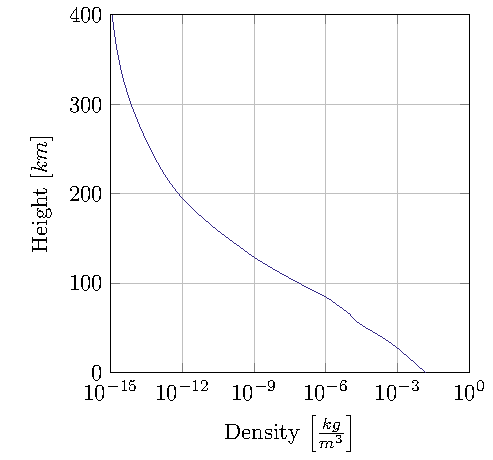
\includegraphics[width=0.95\textwidth]{Figure/Atmosphere/rho_h_180_0.pdf}
		\caption{The atmospheric density} 
		\label{fig:atmos_height_rho}
	\end{subfigure}
	\begin{subfigure}{0.48\textwidth}
		\centering
		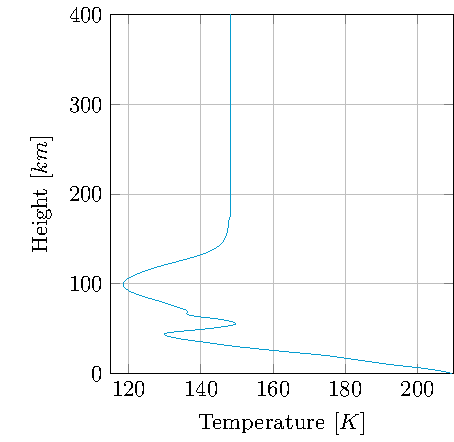
\includegraphics[width=0.95\textwidth]{Figure/Atmosphere/T_h_180_0.pdf}
		\caption{The atmospheric temperature}
		\label{fig:atmos_height_T}
	\end{subfigure}
	\caption{The atmospheric properties for different heights}
	\label{fig:atmos_height}
\end{figure}

Changes in atmospheric properties also occur across the different longitudes and latitudes. These changes are not used in the analysis of the trajectory through the atmosphere and should be considered in further design stages. The differences in density in lower parts of the atmosphere (lower than approximately 100 $[km]$) can be $30\%$ between the highest and lowest density found at a latitude of 0 $[deg]$. The density at 4 different heights is portrayed in Figure \ref{fig:atmos_density_heights}. In order to reduce the maximum error, in the trajectory calculation the latitude is used for which the density profile most closely mimics the average density over the longitudes. This longitude is chosen to be $180 \left[^\circ\right]$.


\begin{figure}[h]
	\centering
	\begin{subfigure}{0.49\textwidth}
		\centering
		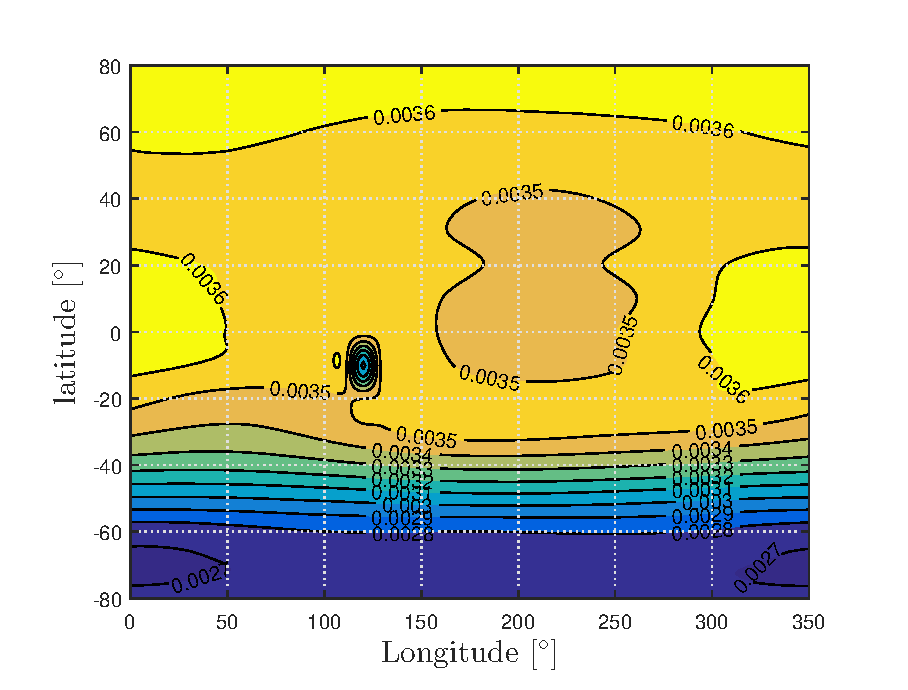
\includegraphics[width=0.98\textwidth]{Figure/Atmosphere/density_15km.eps}
		\caption{15 $[km]$} 
		\label{fig:atmos_rho_15km}
	\end{subfigure}
	\begin{subfigure}{0.49\textwidth}
		\centering
		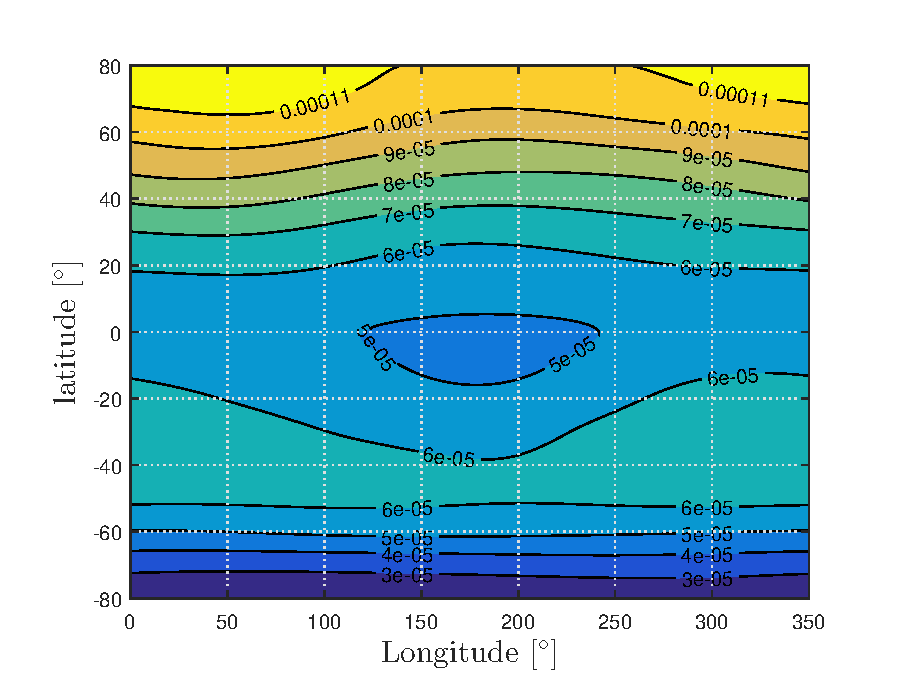
\includegraphics[width=0.98\textwidth]{Figure/Atmosphere/density_50km.eps}
		\caption{50 $[km]$} 
		\label{fig:atmos_rho_50km}
	\end{subfigure}
	\begin{subfigure}{0.49\textwidth}
		\centering
		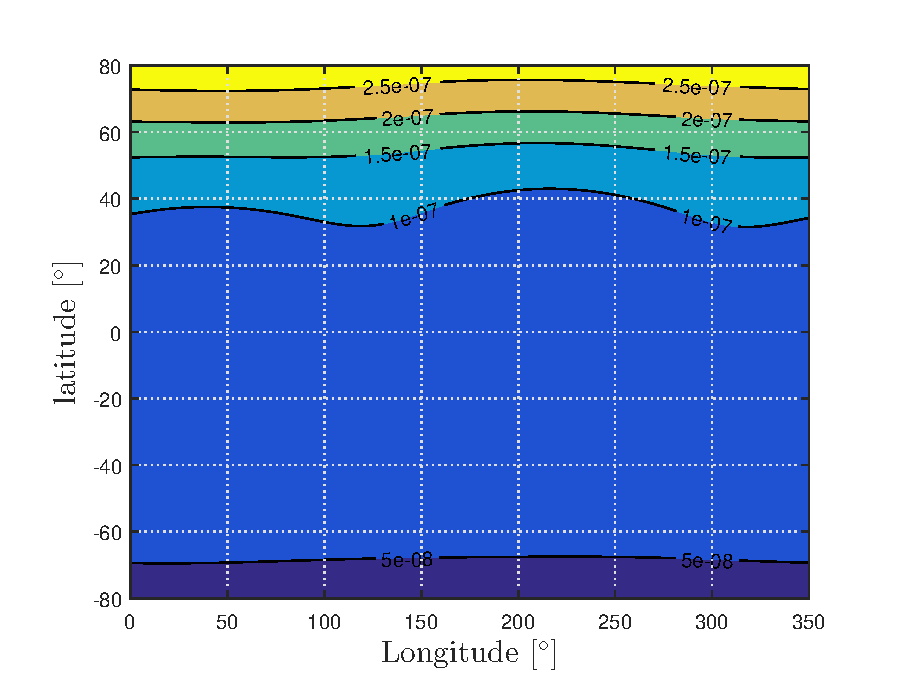
\includegraphics[width=0.98\textwidth]{Figure/Atmosphere/density_100km.eps}
		\caption{100 $[km]$} 
		\label{fig:atmos_rho_100km}
	\end{subfigure}
	\begin{subfigure}{0.49\textwidth}
		\centering
		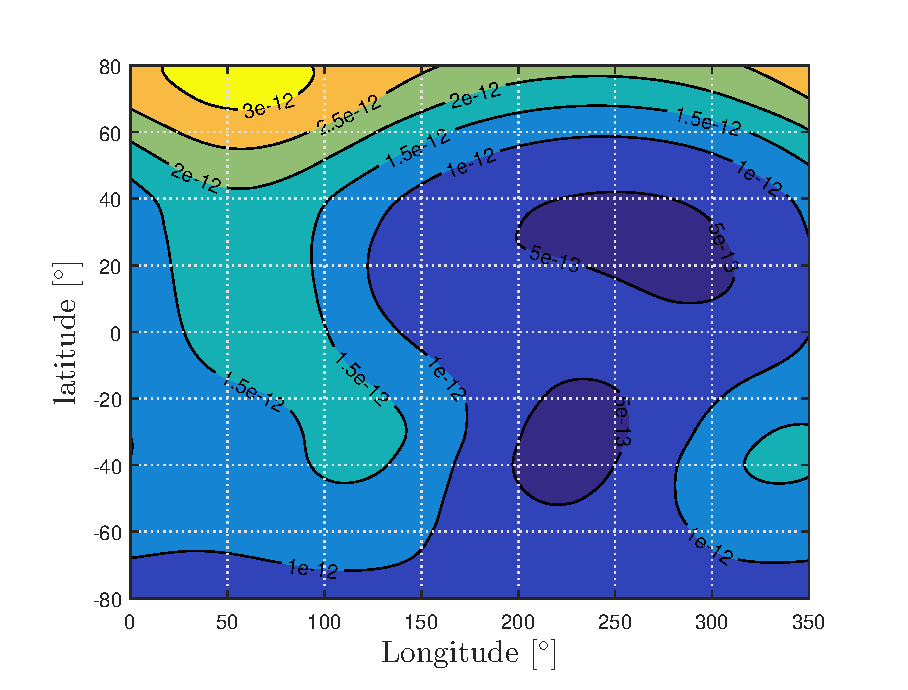
\includegraphics[width=0.98\textwidth]{Figure/Atmosphere/density_200km.eps}
		\caption{200 $[km]$} 
		\label{fig:atmos_rho_200km}
	\end{subfigure}		
	\caption[Atmospheric density as a function of latitude and longitude]{Atmospheric density as a function of latitude and longitude, for different heights}
	\label{fig:atmos_density_heights}
\end{figure}
